\chapter{Berechenbarkeitstheorie}
\begin{center}
	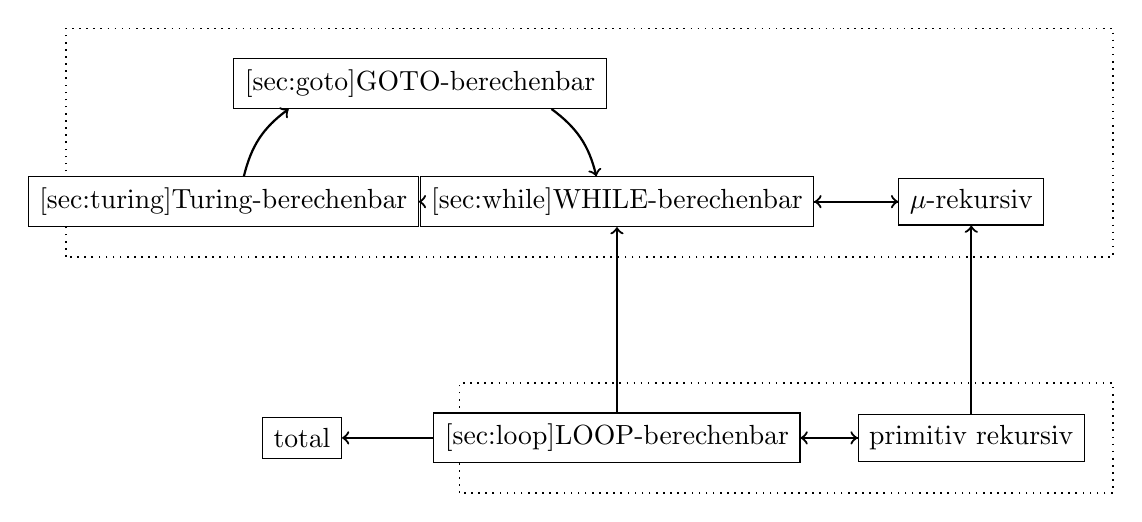
\begin{tikzpicture}
		\tikzset{
			grouplabel/.style={
				draw,
				fill = white,
				rectangle,
				inner sep = 4pt,
			}
		}

		\draw [dotted, line width=0.2mm] (0,6.3) rectangle (13.3,9.2);
		\draw node (tm) at (2,7) [grouplabel] {\hyperref[sec:turing]{Turing-berechenbar}};
		\draw node (while) at (7,7) [grouplabel] {\hyperref[sec:while]{WHILE-berechenbar}};
		\draw node (goto) at (4.5,8.5) [grouplabel] {\hyperref[sec:goto]{GOTO-berechenbar}};
		\draw node (mu) at (11.5,7) [grouplabel] {$\mu$-rekursiv};
		\draw [dotted, line width=0.2mm] (5,3.3) rectangle (13.3,4.7);
		\draw node (loop) at (7,4) [grouplabel] {\hyperref[sec:loop]{LOOP-berechenbar}};
		\draw node (prek) at (11.5,4) [grouplabel] {primitiv rekursiv};
		\draw node (total) at (3,4) [grouplabel] {total};

		\draw[thick, ->] (while) to (tm);
		\draw[thick, ->] (tm) to[bend left=20] (goto);
		\draw[thick, ->] (goto) to[bend left=20] (while);
		\draw[thick, ->] (mu) to (while);
		\draw[thick, ->] (while) to (mu);

		\draw[thick, ->] (prek) to (mu);
		\draw[thick, ->] (loop) to (while);
		\draw[thick, ->] (loop) to (prek);
		\draw[thick, ->] (prek) to (loop);

		\draw[thick, ->] (loop) to (total);
	\end{tikzpicture}
\end{center}


\section{Turing-Berechenbarkeit}\label{sec:turing}
Eine Funktion $f:\N^k\rightarrow \N$ heißt Turing-berechenbar, falls eine deterministische Turingmaschine existiert, die $f(n_1,\ldots,n_k)=m$ berechnet indem, sie gestartet auf dem $k$-Tupel $(n_1,\ldots,n_k)$ nach endlich vielen Berechnungsschritten einen Endzustand erreicht und dann $m$ auf dem Band steht.


\section{LOOP-Berechenbarkeit}\label{sec:loop}
Eine Funktion $f:\N^k\rightarrow \N$ heißt LOOP-berechenbar,  falls es ein LOOP-Program $P$ gibt, das gestartet auf der Eingabe $n_1,n_2,\ldots,n_k$ in den Variablen $x_1,x_2,\ldots,x_n$ nach endlich vielen Schritten hält und die Variable $x_0$ den Wert $f(n_1,\ldots,n_k)$ beinhaltet.
\subsection{Erlaubte Anweisungen}
\begin{itemize}
	\item Wertzuweisungen: $x_i\coloneqq x_j$ und $x_i\coloneqq c$
\end{itemize}



\section{WHILE-Berechenbarkeit}\label{sec:while}
\subsection{Erlaubte Anweisungen}

\section{GOTO-Berechenbarkeit}\label{sec:while}
\subsection{Erlaubte Anweisungen}
